\documentclass[12pt]{article}
\usepackage{amsmath}
\usepackage{csvsimple}
\usepackage{graphicx}
\graphicspath{ {./../images/} }
\usepackage{hyperref}
\usepackage[latin1]{inputenc}
\usepackage{listings}

\DeclareMathOperator{\Tr}{Tr}

\lstset{
  columns=fullflexible,
  breaklines=true,
}

\title{El Farol Bar Problem on a Social Network}
\author{Rebecca Cohen}

\begin{document}
\maketitle
\section{Abstract}
Does network structure determine which agents will attend the bar in a modified El Farol Bar problem.  In most cases, the network does not appear to converge to a single stable fixed point, but rather oscillates around an attractor in which some agents always attend and others attend in alternating weeks.  

\section{Introduction}
Motivate El Farol bar problem.  Work with social networks.

\section{Social Decision Function}
To test the hypothesis that local differences in the structure of social networks can encode the diversity of strategies required to regulate attendance, we construct a simple scenario in which each agent chooses to attend the bar if at least $\ell$ of the agent's neighbors attended the previous week.  We define the attendance vector $\vec{y}(t)$ such that
\begin{equation}
  y_i(t) = \begin{cases}
    1 &\text{if agent}\; i \; \text{attends on week t} \\
    0 &\text{otherwise}
  \end{cases}
\end{equation}

Then 
\begin{equation}
  \vec{y}(t + 1) = F(\mathbf{A}\vec{y}(t))
\end{equation}

where
\begin{equation}
  F(\vec{x})_i = \begin{cases}
    1 &\text{if} \; x_i > \ell \\
    0 &\text{otherwise}
  \end{cases}
\end{equation}

A traditional implementation of the El Farol bar problem would require some mechanism for modulating attendance patterns depending on the congestion level at the bar.  However, this paper will focus on the regulatory effect of the network structure itself.  As we shall see, in many cases the interaction of network structure with an appropriate choice of $\ell$ will maintain attendance below the traditional 60\% threshold. 

Fixed points of this system occur where

\begin{equation}
  \vec{y}_{\infty} = F(\mathbf{A}\vec{y}_{\infty})
\end{equation}

Unsurpisingly, the trivial fixed point of $\vec{y}_{\infty} = \vec{0}$ is a solution since $\mathbf{A}\vec{0} = \vec{0}$ and $F(\vec{0}) = \vec{0}$.  There may also be nontrivial fixed points, depending on the network and $\ell$.  Let $S$ denote a subset of nodes such that every element of $S$ has at least $\ell$ neighbors in $S$ and no element of $S^C$ has $\ell$ neighbors in $S$.  If we construct $\vec{y}$ such that  
\begin{equation}
  y_i = \begin{cases}
    1 &\text{if} \; i \in S \\
    0 &\text{otherwise}
  \end{cases}
\end{equation}
 then for all $i \in S$, $\mathbf{A}\vec{y} > \ell$ and for all $y \notin S$, $\mathbf{A}\vec{y} \leq \ell$.  Thus $\vec{y} = \mathbf{A}y$. 

In general, we cannot expect $S$ to be unique.  As a simple example, suppose the network contains two mutually exclusive $\ell$-cliques, each of which is connected to the rest of the network by less than $\ell$ edges.  Then the network must have at least 3 nontrivial fixed points, consisting of the vertices in one or both cliques.

However, a finite network must have a unique maximal fixed point (MFP), in which every agent that could possibly be a member of $S$ is.  
TODO: Present MFP algo and show that sol'n is unique (or fuck off). 

TODO: Show that the 0 sol'n is unstable for Erdos-Renyi and configuration model.  Without an analytical description of nontrivial fixed points, it is difficult to understand whether they are stable.  BLABLA  

\section{Deterministic Simulations}
We can use numerical simulations to gain a stronger understanding of the steady state behavior of the system (if applicable).  We use three different well-understood random graph models: the Erdos-Renyi random graph, in which all possible edges exist with equal probability, the Chung-Lu model, which weights edge probabilitiies to obtain a target degree distribution, and the stochastic block model (SBM), in which the probabiliity of an edge is depends on its membership in a particular block.  Comparing the results on the Erdos-Renyi network vs. the Chung-Lu model, generated with a power law degree distribution, allows us to evaluate the impact of a heterogeneous degree distribution on the steady state of the system, while the SBM allows us to explore the impact of community structure.  The simulations were designed so that that the number of nodes and edges would be similar between the three models.  See Appendix for additional implentation details.

Numerical simulations show that weekly attendance numbers reach a fixed point in most but not all trials.  However, even on the same network with the same number of agents attending at $t=0$, weekly attendance varies between trials.  In both the Erdos-Renyi and SBM simulations, some initial conditions (wiith 30\% of agents attending) led to no agents attending at steady state, while others led to attainment of the maximal fixed point.  In addition, there were intermediate states in which a fraction of the MFP attended while other members of the MFP never attended.  These intermediate states were much more frequent on the SBM versus the Erdos-Renyi model. 

In contrast, the Chung-Lu model leads to much more stable results.  However, results are still not identical between trials.  For example, on a network of 300 agents, 141 attended in the steady state for 94\% of trials, while 142 attended the other 6\% of the time.  The MFP contained 153 nodes, and no trial attained the MFP.

Figure BLAH summarizes  attendance

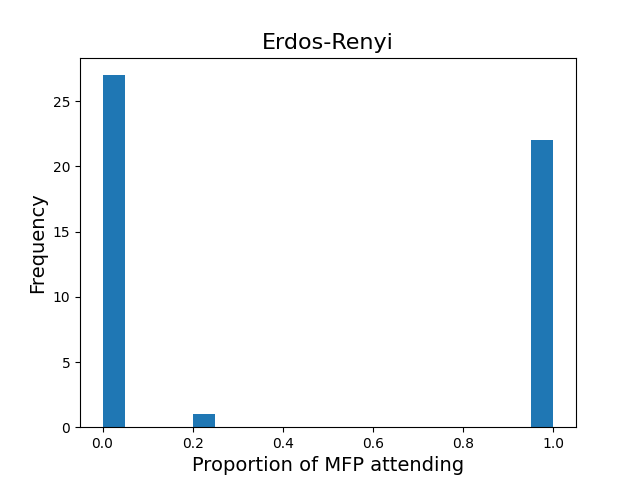
\includegraphics[scale=0.7]{gnp_attendance.png}
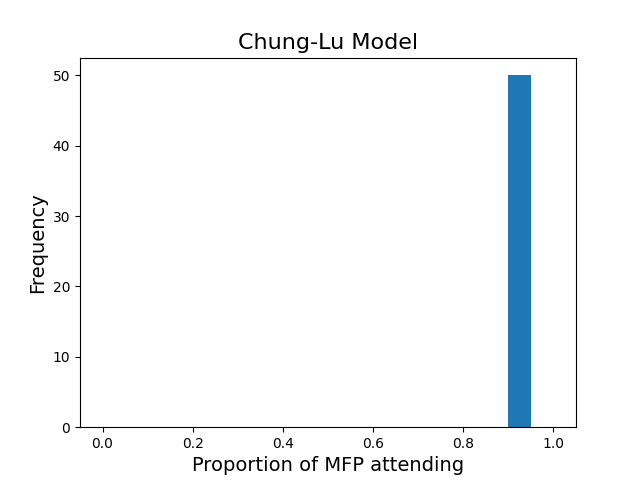
\includegraphics[scale=0.7]{cm_attendance.png}
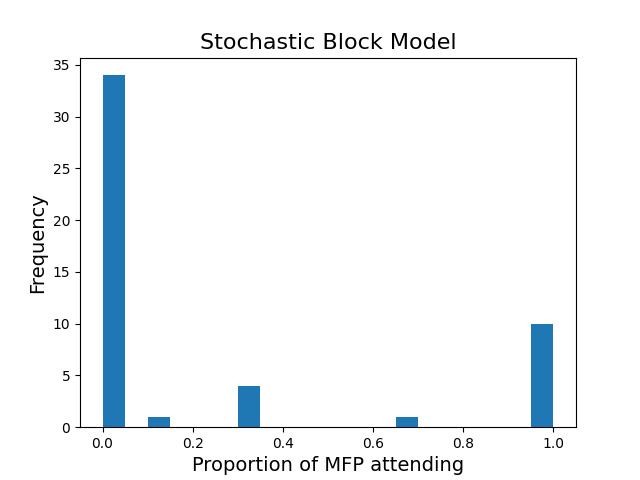
\includegraphics[scale=0.7]{sbm_attendance.png}

In many simulations, the exact same group of agents attended every week, resulting in a true fixed point as described in Section 3.  However, all three experiments had some trials in which the composition of agents attending varied from week to week.  After discarding the first 50 timesteps of the simulation, some agents attended every timestep, some agents never attended, and, in many trials, some agents attended exactly half of the timesteps.  Further investigation revealed that agents attending alternate weeks were coupled to each other.  

In the simplest scenario, a pair of agents ($A_1$ and $A_2$) are neighbors and each have $\ell - 1$ neighbors that always attend.  If agent $A_1$ attends at time $t$, while agent $A_2$ does not, then at time $t+1$, agent $A_2$ will attend, as it had $\ell$ neighbors attending at time $t$, while agent $A_1$ will not attend, as it had just $\ell - 1$ neighbors in attendance at time $t$.  Thus the two agents will toggle back and forth indefinitely, essentially caught in a game of telephone tag in which they miss running into each other at every timestep.  In some cases, more complex interactions occur.  While more agents may be involved, the cycles always have period 2.

\begin{center}
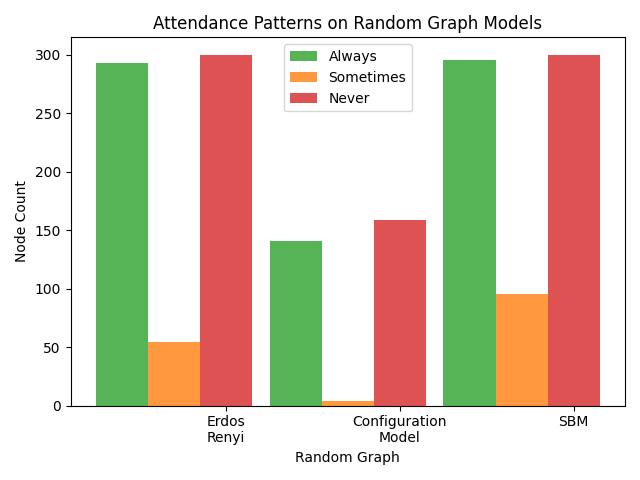
\includegraphics[scale=0.7]{always_sometimes_never.png}
\end{center}

Figure GORP shows the number distinct agents attending always, sometimes, or never in at least one trial for each of the three random graph models.  The figure shows the contrast between the Chung-Lu model with a heavy-tailed degree distribution, which has around half of the nodes in the Always and Never camp, and very few in Sometimes, compared with the Erdos-Renyi and stochastic block models, which have a much more variabiliity.  Almost all agents are occasionally in both the Always and Never groups depending on the trial, and many more agents attend sometimes.  These results suggest that more homogeneous degree distributions increase the probability of agents engaging in telephone tag behaviors, while contributing to more volatile results.  In contrast, the heavier-tailed degree distribution appears to have stabilizing influence on the outcome.

\section{Analysis of Stability on Highly Structured Networks}

To understand the relationship between telephone tag and degree distribution, we consider a much more structured network.  Consider a network with nodes are arranged in a grid of shape $N$ by $N$ for some even integer $N$.  Each node is connected to the other nodes in its Von Neumann neighborhood, defined as the cells to the left, right, above or below where they exist.  Cells on the edges of the grid are have edges wrapping around to connect to the other side, so every node has exactly four neighbors.  If the simulation is run on this network, with $\ell = 3$, meaning a minimum of 4 neighbors are required, both universal attendance and universal nonattendance will be fixed points.  Universal telephone tag, in which every agend attends in alternate weeks, offset from all four neighbors, will also sustain itself indefinitely barring any perturbations.

The system can sustain either universal attendance or universal telephone tag, but has no redundant edges above the minimum required.  If a single node in the universal attendance scenario fails to attend at one timestep, as shown in figure BLEEP, its neighbors will not attend at the next one, and a telephone tag scenario will emerge, beginning at the epicenter of the disruption and spreading across the entire network until there is universal telephone tag.  In the universal telephone tag scenario, as soon as one node fails to attend, non-attendance will spread and engulf the entire network, as show in figure BWOOP.

However, if an agent attends an extra time in either the universal telephone tag or universal nonattendance scenarios, the effect cannot spread and the system returns to equilibrium as shown in figures meh and morp.

On these networks and other $\ell + 1$-regular graphs, universal nonattendance is the only stable fixed point.  The fact that attendance can stabilize to a nonzero level in simulations on random networks is only possible because some nodes have degree greater than $\ell + 1$.

\section{Noise?}
Adding noise allows encourages the telephone tag scenario to synchronize but also allows stable fixed points to erode?  Locally treelike networks with heterogeneous degree distributions may settle into something close to the maximal fixed point.  Punctuated equilibria on SBM.

\section{Discussion and Future Work}

The El Farol Bar problem has traditionally considered a population of agents with diverse strategies attempting to share a limited resource.  Traditional strategies often result in some agents attending always, some attending never, and some attending periodically, with a total attendance close to the tolerance threshold.

In this paper, we find that a population of agents all following the same network-based strategy can behave in a similar way, with a subset of agents always attending, a subset never attending, and a subset attending periodically.  Furthermore, we have seen how network topology and the inclusion of noise influence the outcomes.

In addition to exploring a classic game theory problem with a new twist, this work has interesting parallels with opinion modeling.  Spread of trends, social media hashtags.  Hipster effect.

A natural extension of this work would be to allow agents to evolve their strategies toward improving their utiility.  In this scenario, an agents' behavior would depend not only on the topology of the neighborhood but on the distribution of strategies within it.  It could also be interesting to examine the results of these processes on empirical social network datasets, which tend to be much less locally treelike than the random graph models examined.    

\section*{Code}

\end{document}